\section{Séance 5 - Réglage de la sensibilité}
\subsection{Objectif}
Durant la séance 4, la valeur du déphasage a été calculée pour optimiser la linéarité
de la réponse du système. Il a également été possible de calculer la sensibilité du système
à ce déphasage.
\vspace{0.2cm}

Le but de cette séance sera donc de modifier le gain du système pour obtenir une sensibilité de
10 V/mm. L'offset du système sera ensuite ajusté pour obtenir une tension de 0 V à la position
de repos.
\vspace{0.2cm}

\subsection{Théorie}
Pour obtenir la sensibilité souhaitée, il convient de modifier le gain du filtre passe bas
de notre système.

\begin{figure}[H]
    \centering
    \includegraphics[width=10cm]{Images/Seance5/Gain système.png}
    \caption{Circuit du filtre passe bas}
    \label{fig:FPB}
\end{figure}

La résistance $R_{14}$ ayant une valeur de 0 $\Omega$, le gain de ce système est défini comme suit :

\begin{equation*}
     |K| = \frac{R_{10}}{R_{13}}
\end{equation*}

Il est cependant également possible d'écrire le gain en fonction de l'entrée et de la sortie du
système :

\begin{equation*}
    |K| = \frac{S_{out}}{S_{in}}
\end{equation*}

Connaissant la sensibilité d'entrée ainsi que celle voulue en sortie, il est possible, en fixant
la valeur d'une résistance, de calculer la valeur de la seconde. La valeur de R$_{10}$ a été fixée
à 10 k$\Omega$. Il est donc possible de calculer le tableau suivant :


\begin{table}[H]
    \centering
    \begin{tabular}{|l|rl|}
    \cline{1-3}
    S$_{in}$  & 0,3023    & V/mm    \\ \hline
    S$_{out}$ & 10         & V/mm    \\ \hline
    K    & 33,08 &  \\ \hline
    R$_{10}$  & 10      & k$\Omega$     \\ \hline
    R$_{13}$  & 302,3     & $\Omega$     \\ \hline
    \end{tabular}
    \caption{Résumé des valeurs calculées}
    \label{tab:ResumeValeurs}
    \end{table}

Pour l'ajustement de l'offset, il sera uniquement fait de manière expérimentale.

\subsection{Manipulation}
Dans un premier temps, deux résistances ont été mises en série afin d'obtenir la résistance
R$_{13}$. Cette nouvelle résistance a été installée sur l'emplacement R$_{13}$

\begin{table}[H]
    \centering
    \begin{tabular}{|l|r|}
    \cline{1-2}
    R$_{1}$   & 270 $\Omega$   \\ \hline
    R$_{2}$   & 32  $\Omega$        \\ \hline
    R$_{1+2}$ & 302 $\Omega$ \\ \hline
    R$_{13_{mes}}$ & 298.7 $\Omega$ \\ \hline
    \end{tabular}
    \caption{Résumé des valeurs calculées}
    \label{tab:ResumeValeurs}
\end{table}

Le gain réel sera donc:
\begin{equation*}
    |K_{reel}| = \frac{R_{10}}{R_{13_{mes}}} = 33.48   
\end{equation*}

Qui donnera une sensibilité réelle en sortie de conditionneur de:

\begin{equation*}
    S_{out} = |K_{reel}|\cdot S_{in} =10.12 \text{ V/mm} 
\end{equation*}
\vspace{0.2cm}

Le jumper J6 a été enlevé puis le potentiomètre a été utilisé pour régler l'offset sur la tension 
de sortie. Pour une distance à la cible de 0.7 mm, une tension de sortie de 0 V est souhaitée.
\vspace{0.2cm}

La tension de sortie a ensuite été mesurée à toutes les positions, pour un déphasage de 0°.
\begin{figure}[H]
    \centering
    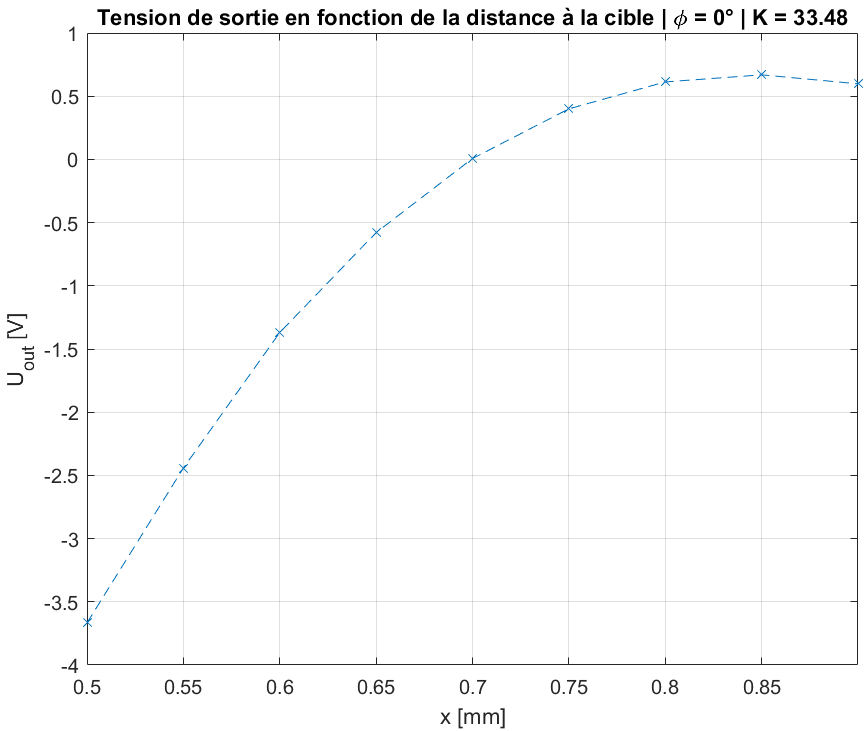
\includegraphics[width=15cm]{Images/Seance5/uout1.png}
    \caption{Tension de sortie à déphasage nul}
    \label{fig:uout1}
\end{figure}

En première instance, il est possible d'observer que la tension de sortie n'est pas linéaire en
fonction de la distance, contrairement à ce qui est attendu. 

\vspace{0.2cm}

En remesurant des valeurs de tension en fonction de la distance à la cible pour plusieurs déphasages,
il a été possible d'observer un comportement qui semblait linéaire pour un déphasage de 120°.

\begin{figure}[H]
    \centering
    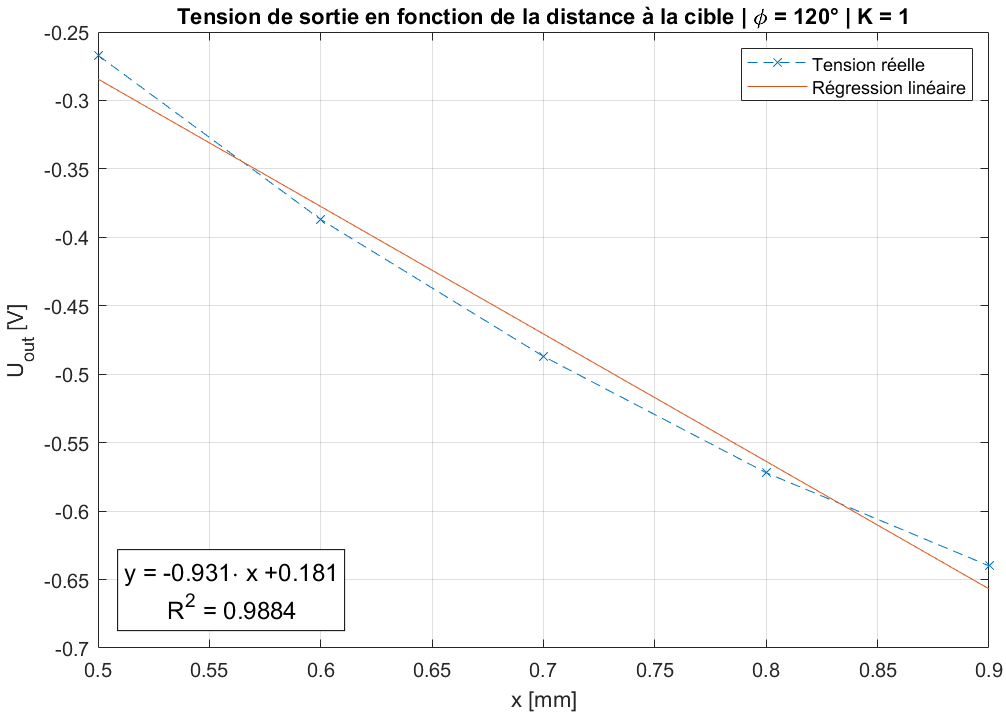
\includegraphics[width=15cm]{Images/Seance5/uout2.png}
    \caption{Tension de sortie à déphasage 120°}
    \label{fig:uout2}
\end{figure}

Le gain ainsi que la résistance $R_{13}$ ont ensuite été recalculés pour les valeurs mesurées :
\begin{equation*}
    |K_2| = \frac{10}{0.931} = 10.74
\end{equation*}
\begin{equation*}
    R_{13} = \frac{R_{10}}{|K_2|}= \frac{10^4}{10.74}= 931\text{ }\Omega
\end{equation*}

Par manque de rigueur et une volonté de vitesse, une résistance d'une valeur de 1 k$\Omega$
a été utilisée pour $R_{13}$. Le gain sera donc de 10 et la sensibilité devrait être de -9.31 V/mm.
\vspace{0.2cm}

Lors du réglage de l'offset, le potentiomètre ne permettant pas d'atteindre une tension de 0 V à
0.7 mm, 180° ont été ajoutés au déphasage. Cette manipulation ne devrait pas changer le comportement
du système autrement que de multiplier la sensibilité par -1, puisque le système est $\pi$ périodique.
L'offset a ensuite pu être compensé.
\vspace{0.2cm}

La sensibilité devrait donc être de 9.31 V/mm.

\begin{figure}[H]
    \centering
    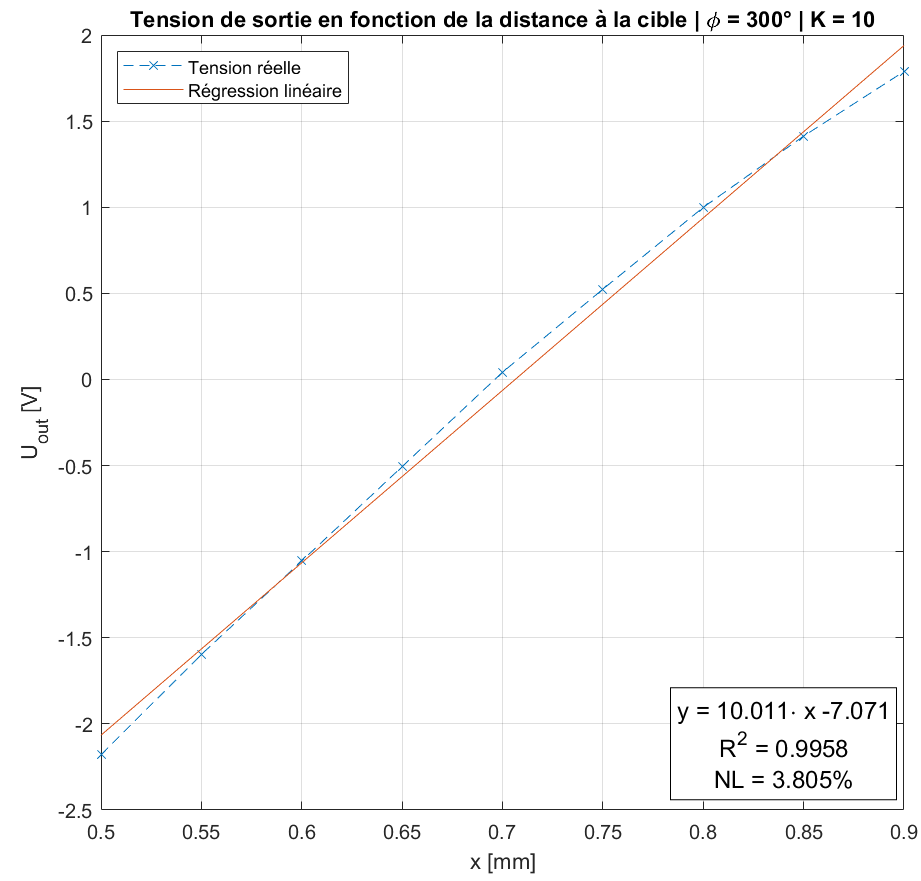
\includegraphics[width=15cm]{Images/Seance5/uout3.png}
    \caption{Tension de sortie à déphasage 300°}
    \label{fig:uout3}
\end{figure}

Bien qu'il soit possible de voir que la tension réelle en fonction de la position n'est pas 
parfaitement linéaire, cette dernière, à contrario de la première itération, s'en approche assez
pour être utilisable.

\subsection{Analyse}
Dans un premier temps, la première manipulation. Comme brièvement expliqué précédemment, la tension
de sortie en fonction de la distance à la cible n'est pas comme attendue. Lorsque l'erreur de
non-linéarité est calculée pour ces valeurs, la valeur suivante est trouvée:
\begin{equation*}
    NL_{\phi=0} = 21.6\% 
\end{equation*}

Ce qui diffère des 0.47\% attendus de manière significative. Cette différence indique que les 
observations faites durant la séance 4 sont probablement correctes, respectivement que les valeurs
obtenues sont aberrantes.
\vspace{0.2cm}

En ce qui concerne la seconde itération, la courbe est relativement linéaire. Il est cependant
possible d'observer une certaine courbure sur la droite. Il est donc probable que le déphasage
trouvé par itération ne soit pas le déphasage optimal. Dans l'idéal, il faudrait refaire la
séance 4 afin d'avoir un nouveau set de données permettant de déterminer proprement le déphasage
optimal.
\vspace{0.2cm}

La sensibilité étant
équivalente à la pente de la droite, il est possible de savoir, grâce à la régression linéaire,
que la sensibilité est de 10.011 V/mm. Malgré une expérimentation un peu hâtive, il est possible
de remarquer que la sensibilité est proche de celle voulue. Cela est probablement dû à la chance.
En effet, les séries de résistances ayant une certaine tolérance, il est possible que $R_{10}$ ait
été plus élevée et $R_{13}$ plus basse qu'attendu. Cette légère différence aurait pu augmenter le
gain, ce qui a permis d'avoir la sensibilité voulue.
\vspace{0.2cm}

Le calcul de la non-linéarité donne la valeur suivante :
\begin{equation*}
    NL_{\phi =300} = 3.805\% 
\end{equation*}

\begin{figure}[H]
    \centering
    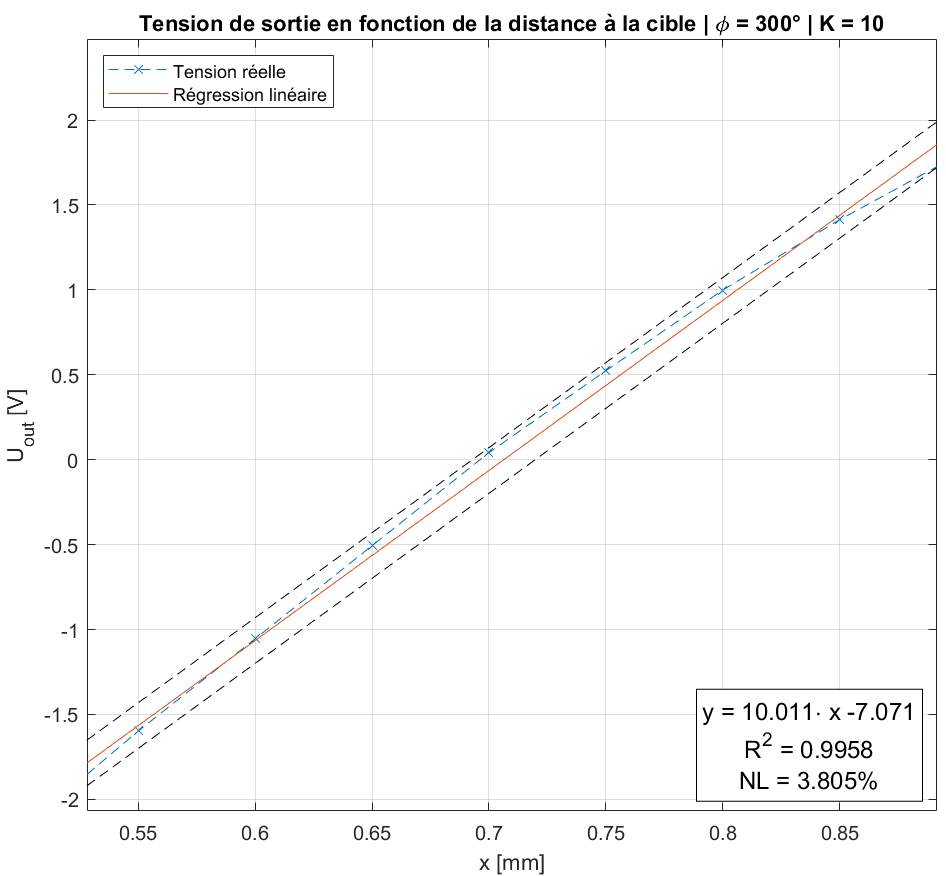
\includegraphics[width=15cm]{Images/Seance5/u_out_enveloppe.png}
    \caption{Tension de sortie à déphasage 300°, avec enveloppe}
    \label{fig:uoutblblb}
\end{figure}


Il est donc possible de considérer que la courbe réelle se trouve dans une enveloppe définie par
l'équation suivante:

\begin{equation}
    U_{out} =  S_{\phi =300} \cdot x + O_{ffset} (1 \pm NL_{\phi =300}) = 10.011\cdot x - 7.071(1 \pm \frac{3.805}{100})
\label{eq:1234}
\end{equation}

Ce qui permet de définir la position en fonction de la tension de sortie :

\begin{equation}
    x = 0.0999 \cdot U_{out}+ 0.7063 \pm 0.0269
    \label{eq:234}
\end{equation}

Cette équation indique plusieurs points intéressants:
\begin{itemize}
    \item Pour une tension mesurée à 0 V, la distance relevée est de 0.7063 $\pm$ 0.0269 mm. Cela
         indique la position de repos.
    \item La sensibilité est de 0.0999 mm/V.
    \item Il existe une incertitude sur la position de 0.0269 mm. 
\end{itemize}
\vspace{0.2cm}

L'équation \ref{eq:1234} étant valable pour des distances à la cible situées entre 0.5 mm et 0.9 mm,
l'équation \ref{eq:234} sera valable pour des valeurs de tensions comprises entre -2.1 V et 2 V.
\subsection{Conclusion}

Cette séance a permis de déterminer que les valeurs prises durant la séance 4 sont aberrantes.
Une recherche itérative a cependant permis de déterminer un déphasage quasi-idéal, trouvé à 300°.
\vspace{0.2cm}

De plus, il a été possible de donner les spécifications intéressantes pour un utilisateur du capteur
couplé à ce conditionneur, pour une cible en cuivre.

\begin{table}[H]
    \centering
    \begin{tabular}{|l|r|}
    \cline{1-2}
    S   & 0.0999 mm/V   \\ \hline
    $O_{ffset}$   & 0.7063  mm        \\ \hline
    $I_{ncertitude}$ & $\pm$0.0269 mm \\ \hline
    Plage de distance & [0.5 : 0.9] mm \\ \hline
    Plage de sortie & [-2.1 : 2.0] V\\ \hline
    \end{tabular}
    \caption{Résumé des valeurs calculées}
    \label{tab:ResumeValeurs}
\end{table}

